\documentclass{classrep}
\usepackage[utf8]{inputenc}
\usepackage{color}
\usepackage{graphicx}

\DeclareUnicodeCharacter{00A0}{~}

\studycycle{Informatyka, studia dzienne, inż I st.}
\coursesemester{IV}

\coursename{Sztuczna inteligencja i systemy ekspertowe}
\courseyear{2023/2024}

\courseteacher{Dr. Krzysztof Lichy}
\coursegroup{poniedziałek, 12:15}

\author{
    \studentinfo{Mateusz Giełczyński}{247662} \and
    \studentinfo{Jakub Kubiś}{247712}
}

\title{Zadanie 1: Piętnastka}

\begin{document}
    \maketitle

    {\color{blue}
    Klasa sprawozdania wymaga następujących pakietów:
        \begin{itemize}
            \item zestaw klas autorstwa Marcina Woli\'nskiego \ppauza u\.zywana jest klasa
            \emph{mwart} (nazwa całego pakietu: \emph{mwcls}),
            \item pakiet \emph{polski},
            \item pakiet \emph{url}.
        \end{itemize}}


%{\color{blue}
%W preambule należy wykorzystać następujące niestandardowe polecenia, aby
%dostarczyć informacje wymagane do wygenerowania sprawozdania:
%\begin{itemize}
%    \item \verb+\studycycle{...}+ \ppauza tryb i rodzaj studiów,
%    \item \verb+\coursesemester{...}+ \ppauza semestr studiów,
%    \item \verb+\coursename{...}+ \ppauza nazwa przedmiotu,
%    \item \verb+\courseyear{...}+ \ppauza bieżący rok akademicki,
%    \item \verb+\courseteacher{...}+ \ppauza prowadzący laboratoria (proszę
%    wpisywać osobę, której oddaje się sprawozdanie, a nie kierownika
%    przedmiotu!),
%    \item \verb+\coursegroup{...}+ \ppauza identyfikator grupy ćwiczeniowej,
%    \item \verb+\studentinfo[e-mail]{imię i nazwisko}{nr albumu}+ \ppauza
%    polecenie wykorzystywane \emph{tylko} w obrębie polecenia \verb+\author+
%    służy do określenia imienia i nazwiska każdego z autorów, jak również
%    numeru albumu i opcjonalnie adresu e\dywiz mail; jeśli adres nie jest
%    podawany, należy pominąć argument opcjonalny.
%\end{itemize}}


    \section{Cel}
    {\color{blue}
    Celem zadania było napisanie programu znajdującego rozwiązanie układanki logicznej zwanej "Pietnastką" oraz zbadanie zasad działania
    algorytmów przeszukujących grafy.
    .}

    \section{Wprowadzenie}
    {\color{red}

    Piętnastka to układanka logiczna składająca się z kwadratowej
    planszy podzielonej na 16 kwadratów. Zawierających cyfry od 1 do 15 oraz jednym miejscem które zawsze pozostaje puste
    co pozwala na przesuwanie sąsiednich kafelków, celem piętnastki jest uporządkowanie kafelków tak aby uzyskać układ liczbowy
    gdzie liczby ułożone są w porządku rosnącym ,a ostatnie pole pozostaje puste.

    \begin{figure}
        \centering
        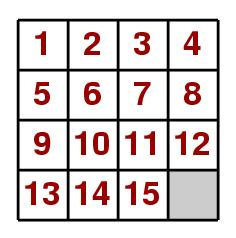
\includegraphics{15}
        \caption{Rozwiązana piętnastka}
    \end{figure}

    Piętnastkę można zinterpretować jako graf, gdzie danym węzłem jest stan planszy. Natomiast krawędzie łączące węzły
    reprezentują możliwe ruchy pomiędzy stanami. Korzeniem w takim grafie będzie początkowy nieroziązany stan układanki.

    Inepretacja piętnastki jako grafu pozwala nam stosować metody przeszukiwania grafów do znajdywania rozwiązań układnaki.
    Zaimplementowane przez nas metody to:
        \begin{itemize}
            \item BFS (breadth-first search) - przeszukiwanie wszerz
                Metoda polega na przeszukaniu wszystkich węzłów na jednej głębokości przed zejściem na niższy poziom.
            \item DFS (depth-first search) - przeszukiwanie wgłąb
                Metoda polega na preszukaniu wszystkich krawędzi danego wierzchołka dopiero po rekurencyjnym przeszukaniu
                wszyskich krawędzi wierzchołków potomnych

            Metoda polega na przeszukiwaniu w głąb, oznacza to że zanim zbada kolejną krawedź pierwszego węzła
            dopiero gdy zbada wszystkie krawędzie kolejnego węzła
            \item A* (A-star)
                Metoda polega na wybieraniu najbardziej obiecujacego węzła na podstawie heurystyki.
                \begin{itemize}
                    \item Heurystyka Hamminga
                        Heurystyka polega na zliczeniu ilości kafelków które nie znajdują się na odpowiednim miejscu.
                    \item Heurystyka Manhattana
                        Heurystyka polega na zliczeniu sumy ruchów, które potrzebuje każdy z kafelków, żeby znależć się na odpowiednim miejscu.
                \end{itemize}
        \end{itemize}

    }

    \section{Opis implementacji}
    {\color{blue}
    Program został stworzony w języku Python 3.
    Klasa Board odpowiada za przechowywanie stanu planszy, związanych z nią informacji oraz
    przemieszczanie elementów planszy.
    Klasa Solver oraz klasy po niej dziedziczące zawierają logikę odpowiedzalną za rozwiązanie układanki daną metodyką.
    Klasa Logger odpowiada za zbieraniu dodatkowych informacji, może być połaczona z klasami rozwiązującymi
    korzystając ze wzorca projektowego obserwatora zaimplemetowanego poprzez klasy ObserverMixin oraz ObservableMixin.

    Powinien się tu również znaleźć diagram UML (diagram klas)
    Jest dobry a jak ci się nie podoba to niech se sam zrobi.
    \begin{figure}
        \centering
        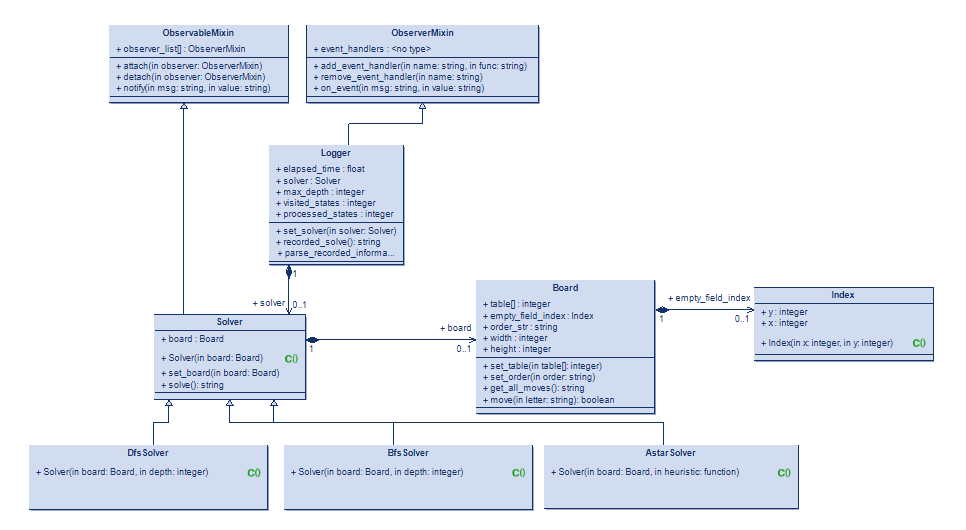
\includegraphics{E:\sise\doc\diagram}
        \caption{}
        \label{fig:}
    \end{figure}


    Należy tu zamieścić krótki i zwięzły opis zaprojektowanych klas oraz powiązań
    między nimi.
        prezentujący najistotniejsze elementy stworzonej aplikacji. Należy także podać,




    }

    \section{Materiały i metody}
    {\color{blue}
        Do przeprowadzenia eksperymentów użyliśmy skryptów oraz programów dostępnych na Wikampie.

    Do przeprowadzenia eksperymentów użyto narzędzi udostępnionycg na platformie WIKAMP,
    zostały wykorzystane przy:
       \begin{itemize}
            \item Generowaniu stanów układanek do rozwiązania
            \item \item Uruchamianiu wykonanego programu dla wygenerowanych układanek
          \item Weryfikacji poprawności rozwiązań
           \item Podsumowaniu wyników
     \end{itemize}
    Badania zostały przeprowadzone dla wszystkich metod oraz możliwych stanów dla
    głębokości od 1 do 7. Natomiast dla głębokości 15 zbadano przebiegi dla A*(obie heurystki)
    oraz dla DFS(Kolejność RDUL).
    }

    \section{Wyniki}
    {\color{blue}
    Poniżej przedstawiono tabelę zawierające:
     \begin{itemize}
         \item Dane
     \end{itemize}
    Oraz wykresy zawierające
    \begin{itemize}
         \item Dane
     \end{itemize}


    \begin{table}[!ht]
    \centering
    \caption{Średnie wyników dla poszczególnych metod}
    \begin{tabular}{|l|l|l|l|l|l|}
    \hline
        Metoda & Długość rozwiązania & Odwiedzone stany & Przetworzone stany & Maksymalna & Czas[ms] \\ \hline
        DFS & 17,981 & 594031,750 & 404246,947 & 19,544 & 2649,430 \\ \hline
        BFS & 6,131 & 6586,751 & 2036,173 & 6,131 & 79,030 \\ \hline
        A* (hamm) & 6,131 & 1627,387 & 552,886 & 11,058 & 0,853 \\ \hline
        A* (manh) & 6,131 & 24,973 & 8,385 & 6,131 & 0,821 \\ \hline
    \end{tabular}
\end{table}


    \begin{table}[!ht]
    \centering
    \caption{Średnie wyników dla poszczególnych metod dla układanek z głębokością 15.}
    \begin{tabular}{|l|l|l|l|l|l|}
    \hline
        Metoda & Długość rozwiązania & Odwiedzone stany & Przetworzone stany & Maksymalna & Czas \\ \hline
        DFS (RDUL) & 17,700 & 5575634,700 & 3794514,150 & 20,000 & 25442,442 \\ \hline
        A* (hamm) & 15,000 & 519618,550 & 173832,600 & 22,900 & 12693,780 \\ \hline
        A* (manh) & 15,000 & 238,250 & 78,850 & 15,050 & 9,109 \\ \hline
    \end{tabular}
\end{table}
    }




    \section{Dyskusja}
    {\color{blue}

    Na podstawie przeprowadzonych badań można wysunąć następujące wnioski:
    \begin{itemize}
        \item Dla układów w odległościach 1-7 od układu wzorcowego zdecydowanie najgorsze efekty uzyskano przy pomocy metody DFS.
            Objawia się to znacznie dłuższym czasem szukania rozwiązania oraz odjandywaniem rozwiązań losowych a niekoniecznie najkrótszych.
        \item Metoda BFS zawsze znajduje najkrótsze rozwiazanie, jest to spowodowane sposobem działania metody, która
                sprawdza wszyskie mozliwe układy na zadanej głębokości przed sprawdzeniem kolejnej.
        \item Metoda A* również zawsze odnajduje najkrótsze rozwiązanie, do tego metoda zdecydowanie najszybicej odnajdywała poprawne rozwiązanie.
       Różnicę pomiędzy wykorzystanymi heurystykami dla układów z głębokością 1-7 jest znikoma.
        \item Dla układów w odległości 15 od układu początkowego nadal A* okazuje się być najszybszą metodą, odnajdującą najkrótsze rozwiązanie.
        \item Porównując heurystyki Manhattana oraz Hamminga można zauważyć, że Manhattan robi wrażenie dwa razy szybszego.
        \item Metoda DFS również wygenerowała poprawne wyniki, w przeciwieństwie do metody BFS, która przez konieczność zapamiętywania wszyskich wężłów na danej głębokości
            zajmuje zbyt wiele miejsca w pamięci operacyjnej aby ukończyć rozwiązywanie zadania.
    \end{itemize}


    Sekcja ta powinna zawierać dokładną interpretację uzyskanych wyników
    eksperymentów wraz ze szczegółowymi wnioskami z nich płynącymi. Najcenniejsze
    są, rzecz jasna, wnioski o charakterze uniwersalnym, które mogą być istotne
    przy innych, podobnych zadaniach. Należy również omówić i wyjaśnić wszystkie
    napotkane problemy (jeśli takie były). Każdy wniosek powinien mieć poparcie we
    wcześniej przeprowadzonych eksperymentach (odwołania do konkretnych wyników).
    Jest to jedna z najważniejszych sekcji tego sprawozdania, gdyż prezentuje
    poziom zrozumienia badanego problemu.}

    \section{Wnioski}
    {\color{blue}
     \begin{itemize}
        \item A* okazał się najbardziej uniwersalną oraz optmalną metodą przeszukiwania grafów zarówno dla małych jak i duzych odległości układanek od układu wzorcowego.
         \item DFS również był w stanie odnaleźć rozwiązania dla każdego zadanego ułożenia układanki, jednak czas potrzebny na rozwiązanie był znaczie większy,
            w szczególności, w przypadku, gdy długość najkrótszego rozwiazania była znacznie mniejsza niż zadana głębokość poszukiwań.
         \item BFS dobrze poradził sobie z przeszukiwaniem układów o małej odległości od układu wzorcowego, jednak dla dużych odległości okazał się zupełnie bezużyteczny.
     \end{itemize}


    W tej, przedostatniej, sekcji należy zamieścić podsumowanie najważniejszych
    wniosków z sekcji poprzedniej. Najlepiej jest je po prostu wypunktować. Znów,
        tak jak poprzednio, najistotniejsze są wnioski o charakterze uniwersalnym.
    }

    \begin{thebibliography}{0}
        \bibitem{l2short} T. Oetiker, H. Partl, I. Hyna, E. Schlegl.
        \textsl{Nie za krótkie wprowadzenie do systemu \LaTeX2e}, 2007, dost\k epny
        online.
    \end{thebibliography}


\end{document}
